\subsection{Bestimmung der Zeitkonstanten des RC-Gliedes}
Durch Aufnahmen des Auf- oder Entladevorgangs am Kondensator kann
die Zeitkonstante $RC$ bestimmt werden.\\
Hierbei wird ein Oszilloskop verwendet, auf dem die Kondensatorspannung $U(t)$ gegen die Zeit betrachtet wird. \\
Nun werden die Auf- bzw. Entladekurve einzeln mit Hilfe des Digitaloszilloskops fotografiert und später in der Auswertung genauer betrachtet.
\begin{figure}[h]
  \centering
  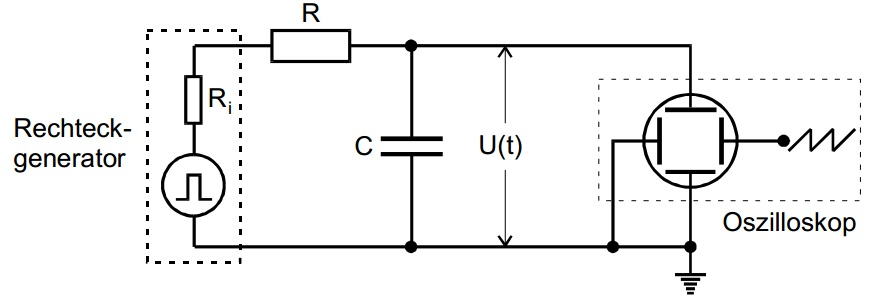
\includegraphics[width=0.7\textwidth]{Grafiken/V353_Abb1.jpg}
  \caption{Messschaltung zur Bestimmung der Zeitkonstanten eines RC-Gliedes durch Beobachtung des 
  Auf- oder Entladevorganges des Kondensators }
  \label{fig:V353_Abb1}
\end{figure}
\subsection{Bestimmung der Amplitude der Kondensatorspannung in Abhängigkeit der Frequenz}

Nun wird die Amplitude ermittelt, indem die Spannung am Kondensator gemessen wird und die Amplitude gegen die Frequenz $f$ im Bereich von 30 bis 100.000 Hz vermessen wird.
\begin{figure}[h]
  \centering
  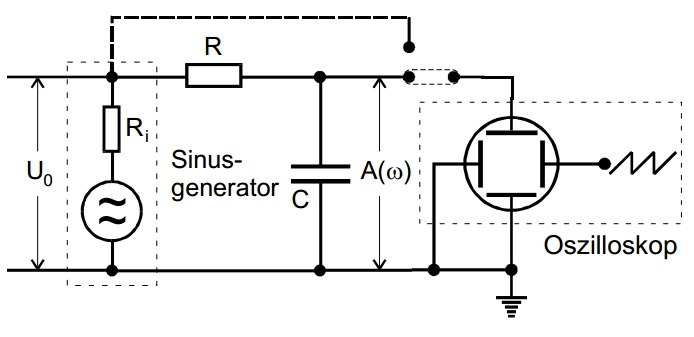
\includegraphics[width=0.7\textwidth]{Grafiken/V353_Abb2.jpg}
  \caption{Messschaltung zur Untersuchung der Frequenzabhängigkeit der Kondensatorspannungsamplitude A in einem RC-Kreis}
  \label{fig:V353_Abb2}
\end{figure}
\subsection{Messung der Phasenverschiebung zwischen Generator- und Kondensatorspannung}

Um die Phasendifferenz $\varphi$ in Abhängigkeit der Frequenz $\omega$
zu bestimmen, werden beide Signale auf jeweils einen Kanal am Oszilloskop gelegt und die Abstände der Perioden für verschiedene Frequenzen gemessen.
\begin{figure}[h]
  \centering
  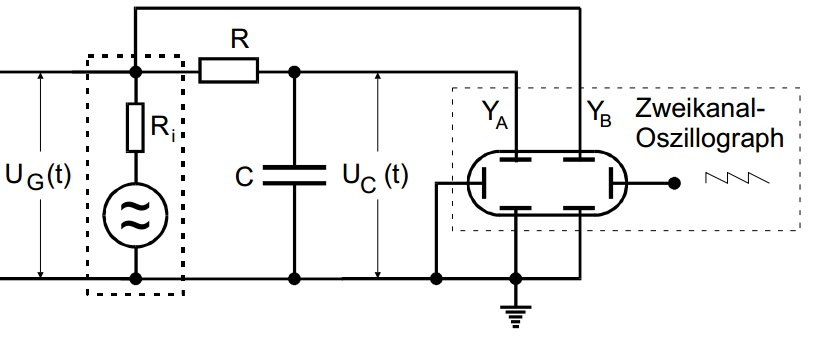
\includegraphics[width=0.7\textwidth]{Grafiken/V353_Abb3.jpg}
  \caption{Schaltung zur Messung der Phasenverschiebung zwischen zwei Spannungen mit einem Zweikanal-Oszilloskop}
  \label{fig:V353_Abb3}
\end{figure}
\subsection{Der RC-Kreis als Integrator}
Für hohe Frequenzen lässt sich feststellen, dass das RC-Glied als Integrator funktioniert.\\
Es werden hier mit dem Oszilloskop die zu integrierende Spannung und die integrierte Spannung angezeigt. Es werden verschiedene Spannungen
eingestellt: Rechteck-, Sinus- und Dreieckspannung und jeweils einzeln aufgenommen.
